\chapter{Pollution control ETIA}\label{appSec:pollution}

In this chapter, additional work on gas emission environmental pollutant characterization is presented. The work was conducted during pyrolysis of digested sludge Lindum (DSL) and measured

Gas measurements have been performed of the gases that are emitted through the chimney. Measurements were performed by the author together with Erlend S\o rmo as an additional learning activity for this master thesis. Measurements included Hg using what instrument, PM10 and syn-gases using FTIR.

The ETIA measurement campaign started September 16, 2021 and aimed to measure emission of environmental pollutants from pyrolysis of the various feedstock types produced at Lindum AS. Included in the campaign are Hg, PM$_{10}$, qualitative analysis of syn-gas using FTIR, quantitative analysis of syn-gas using Low Volume / Medium Volume Sampler LVS / MVS for organic and inorganic pollutants. 


\begin{figure}
    \centering
    \begin{subfigure}[t]{\textwidth}
         \centering
         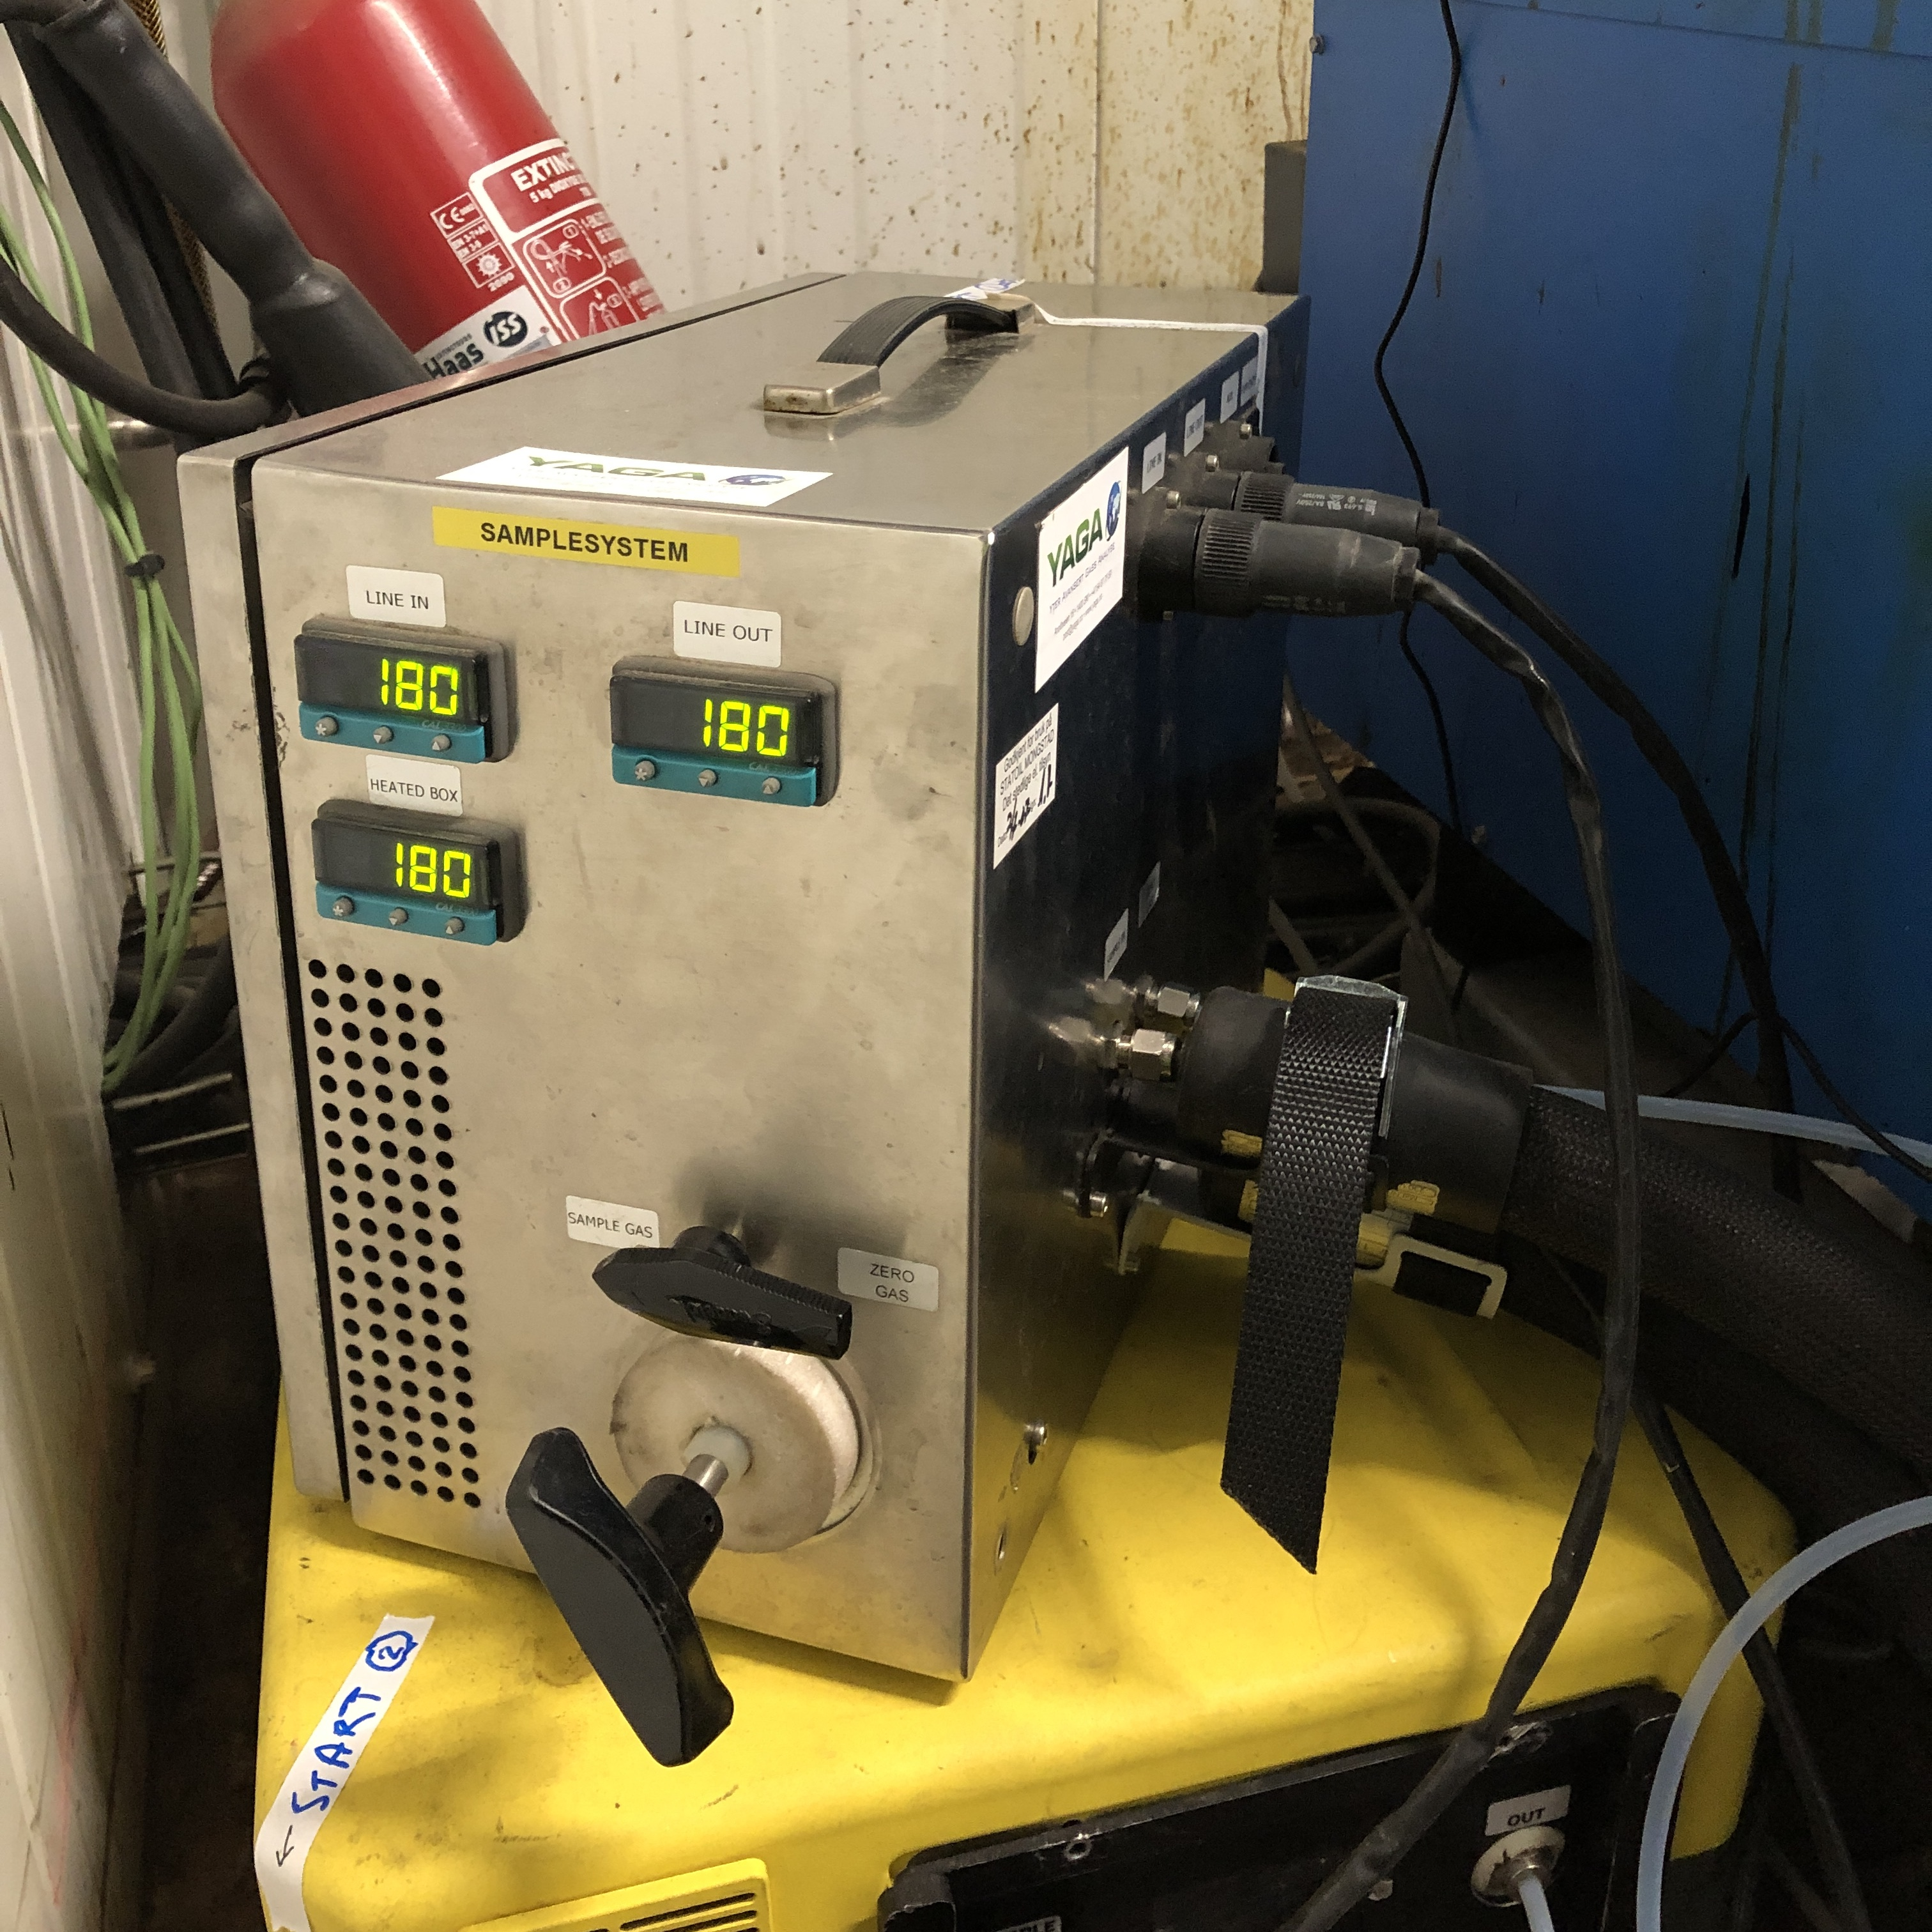
\includegraphics[width=0.6\textwidth]{Bilder/Pyrolysis/FTIR.jpg}
         \caption{}
         \label{appFig:FTIRbox}
     \end{subfigure}
     \hfill
     \begin{subfigure}[t]{\textwidth}
         \centering
         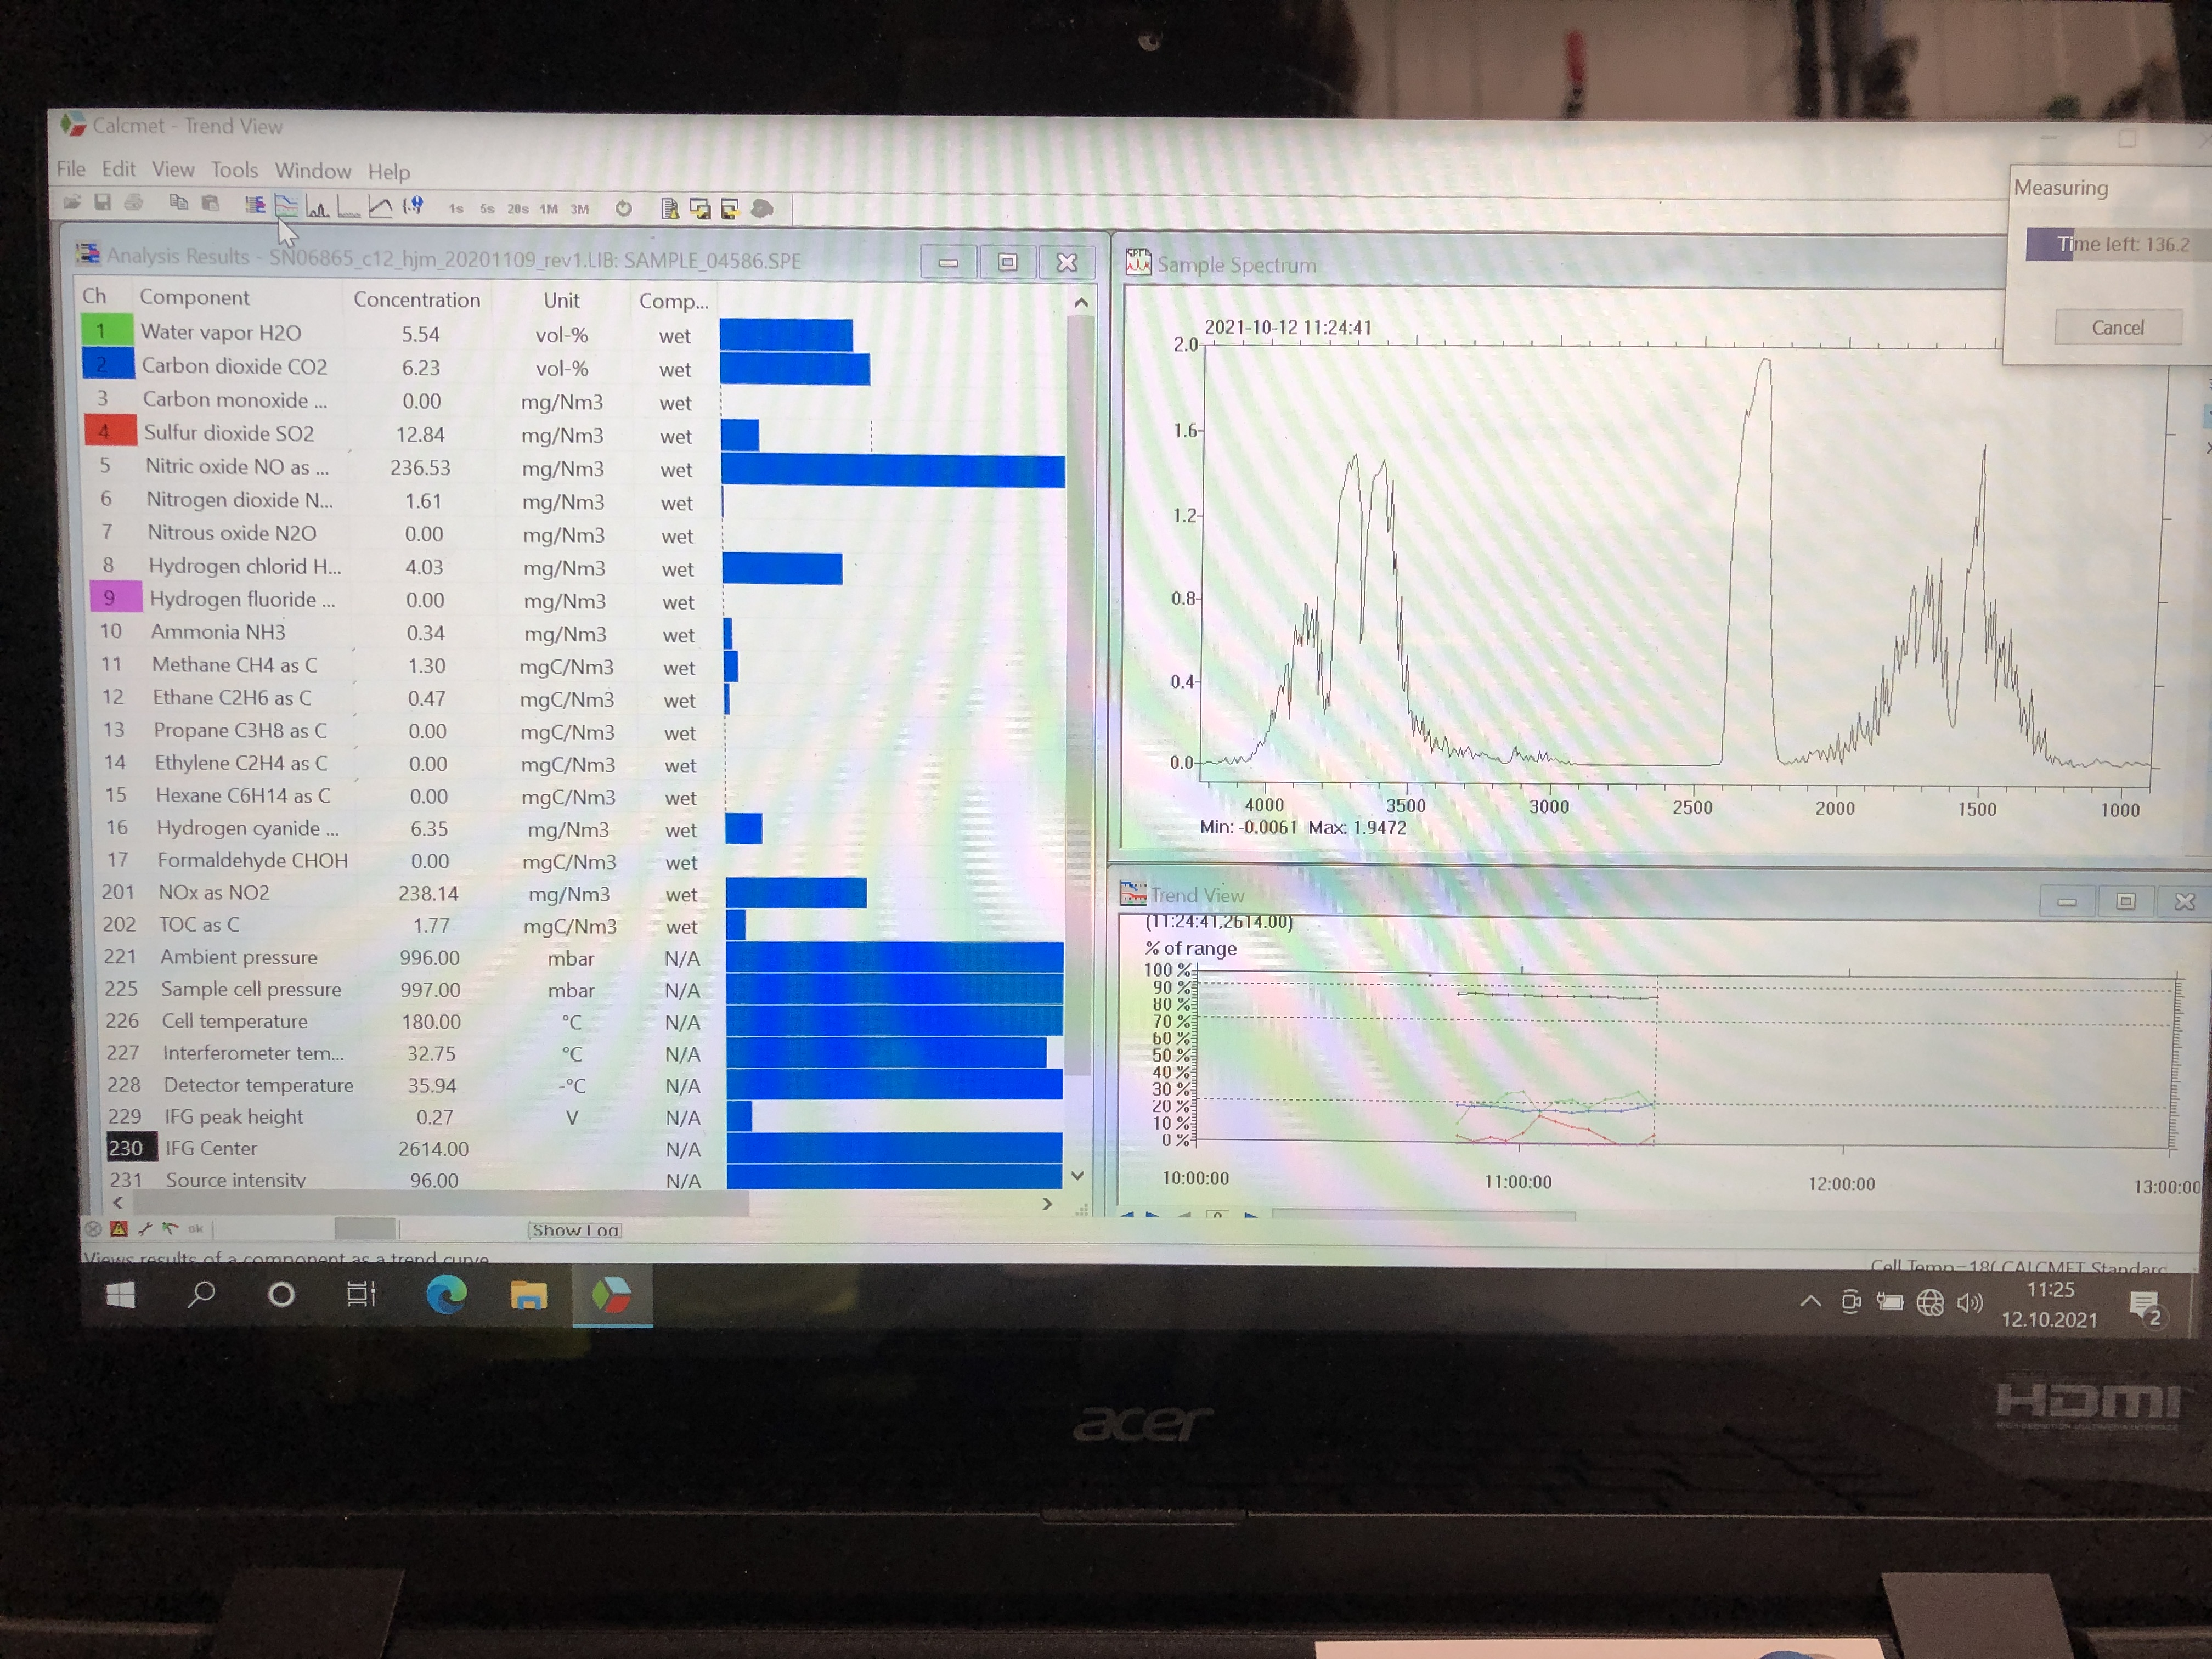
\includegraphics[width=0.6\textwidth]{Bilder/Pyrolysis/FTIRresults.png}
         \caption{}
         \label{appFig:FTIRresults}
     \end{subfigure}
     \hfill
     \caption{(a) FTIR. The tube leading to the FTIR is heated to 180 \textdegree C to prevent condensation of syn-gas. (b) FTIR output results. The results are a screenshot of the FTIR spectra from pyrolysis of Biorest Lindum (BRL).}
    \label{appFig:FTIR}
\end{figure}


\begin{figure}
    \centering
    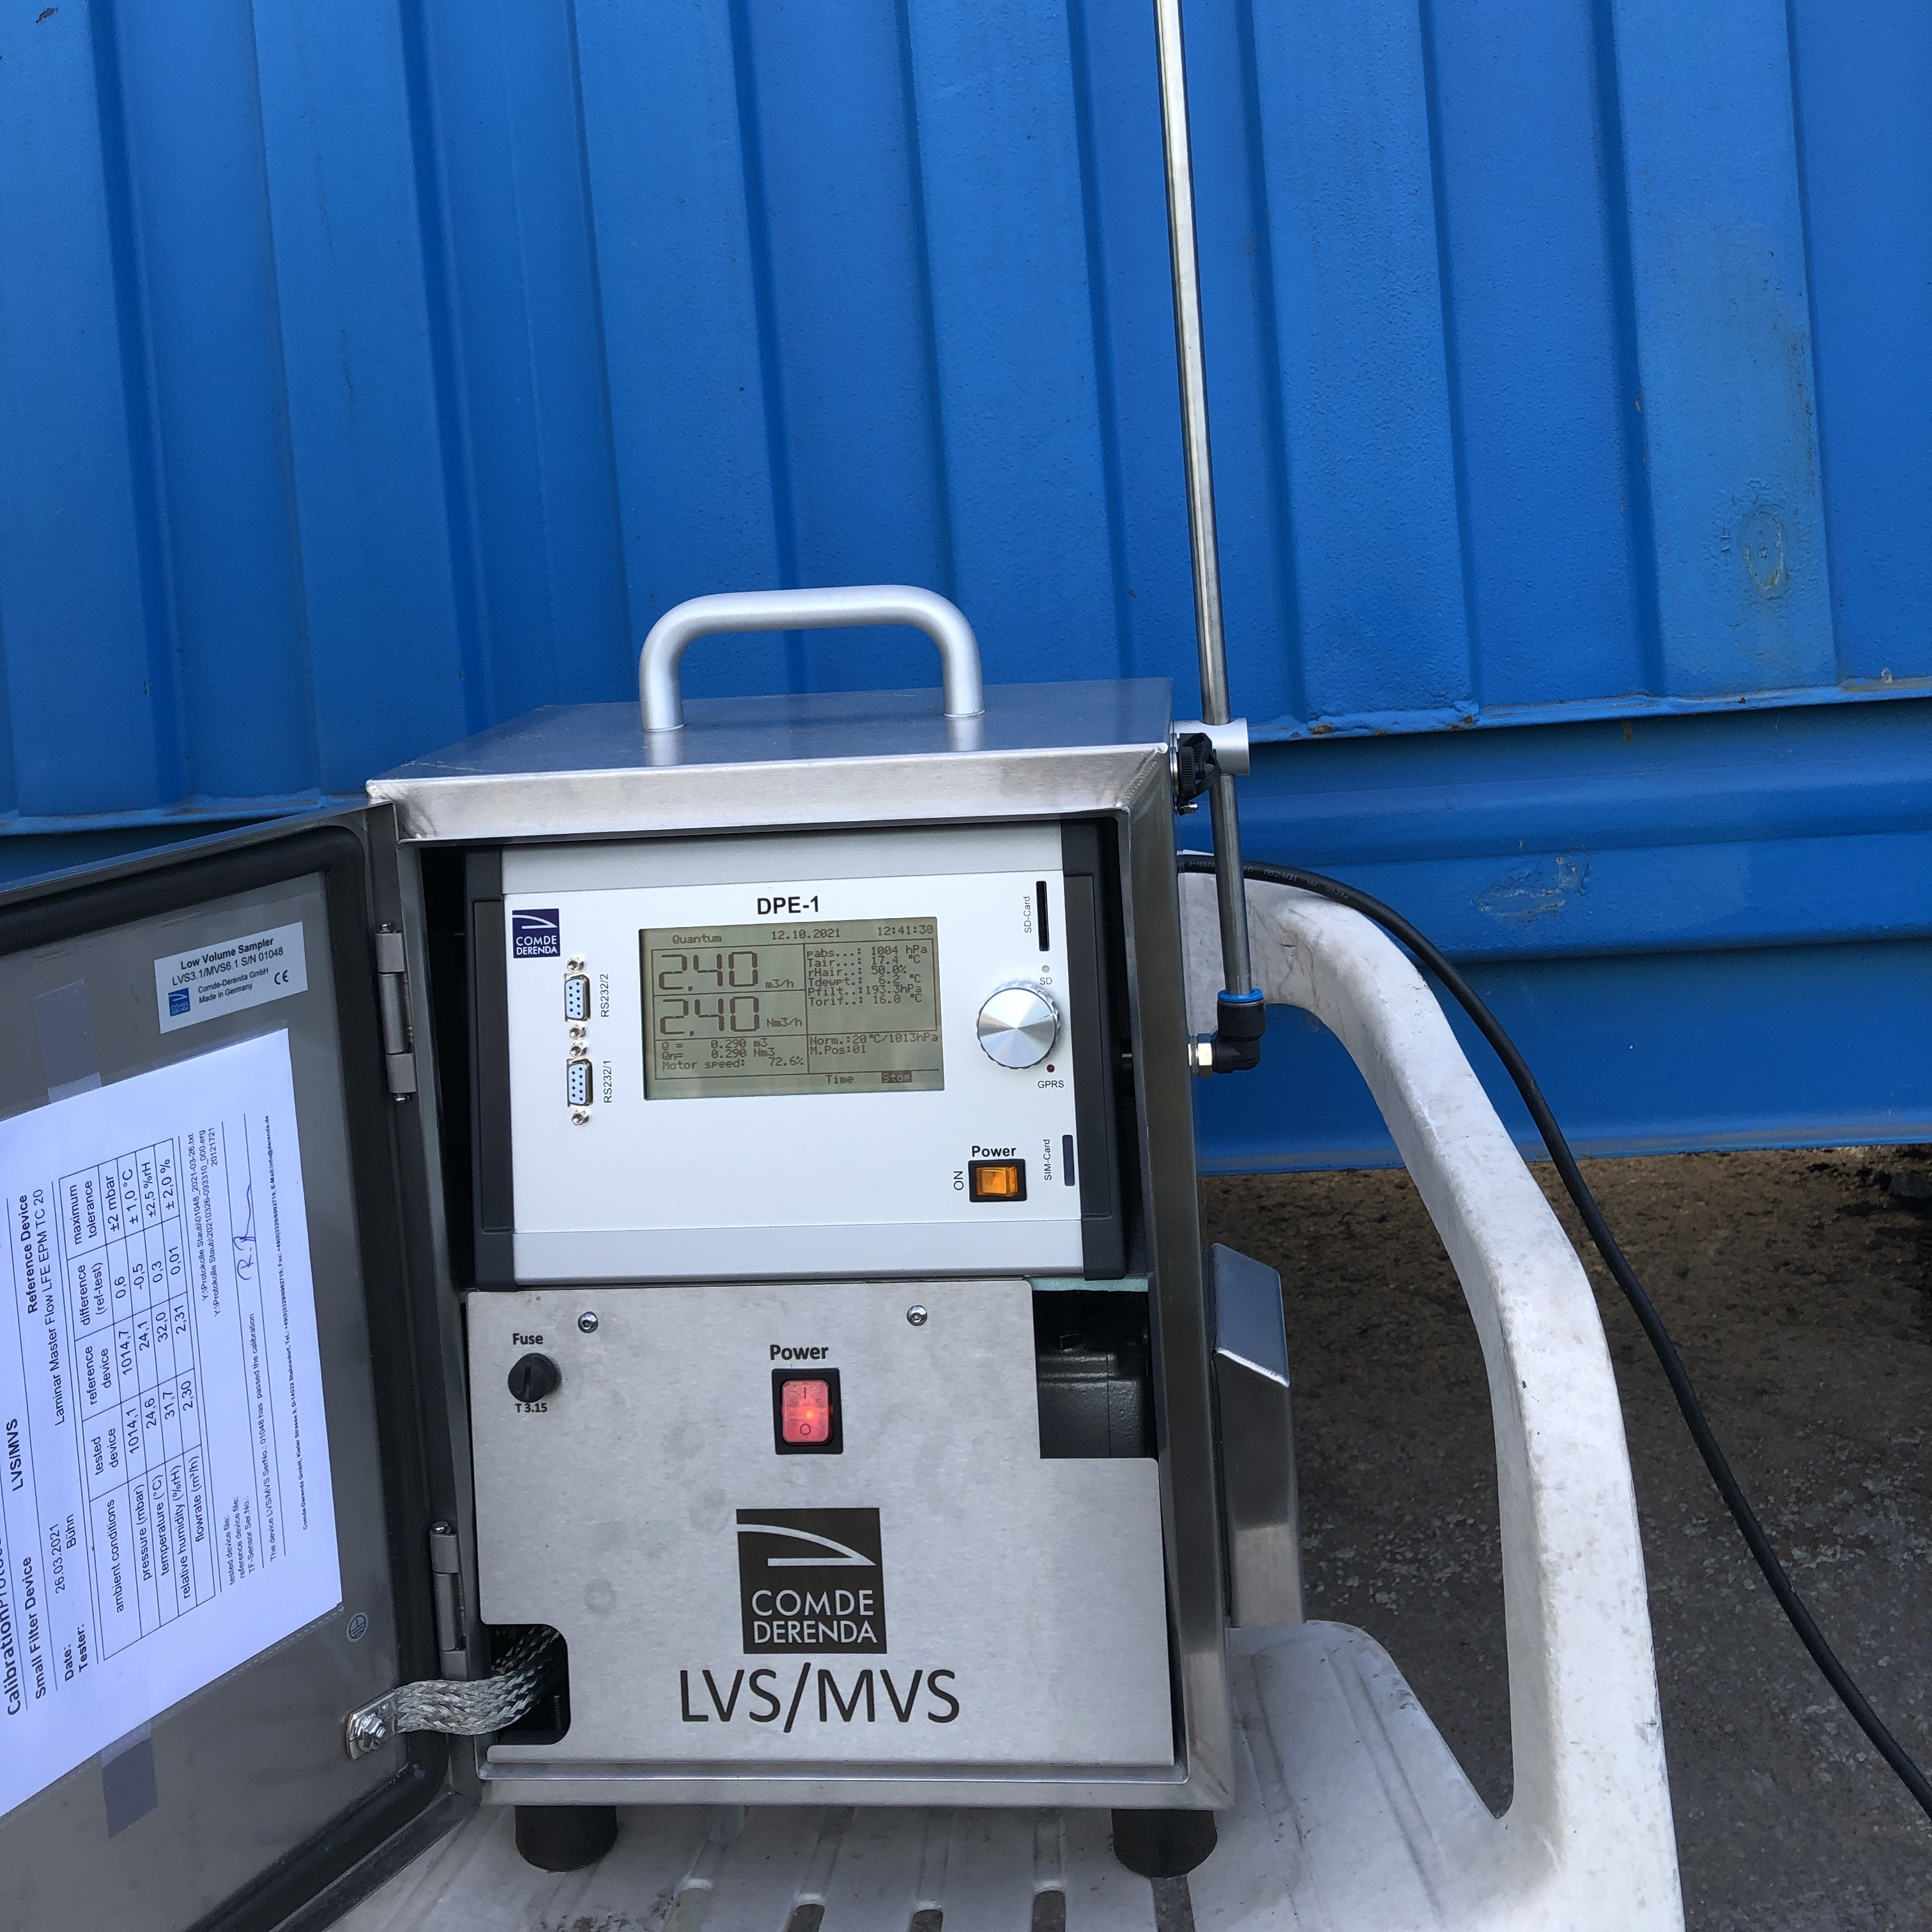
\includegraphics[width=0.85\textwidth]{Bilder/Pyrolysis/ParticlePump.jpg}
    \caption{LVS/MVS vacuum pump draws in air emitted from the ETIA chimney, and the sampler fractionates the airborne fine particles in a sampling inlet. The air containing the desired fine particulate fraction then passes through the filter, where the particles are collected and made available for subsequent gravimetric assessment or analysis. The volumetric flow rate is measured with an orifice plate and electronically adjusted with an accuracy of $\leq$ 2 $\%$. (Copied from comde-derenda.com, bust be rephrased)}
    \label{appFig:ParticlePump}
\end{figure}